\documentclass[10pt]{beamer}
\usepackage{tikz}
\usepackage{pgfplots}
\usepackage{mathtools}
\usepackage{physics}
\usepackage{amsfonts,amsmath,amssymb,amsthm}
\usetikzlibrary{shapes.geometric, arrows}

\tikzstyle{startstop} = [rectangle, rounded corners, minimum width=3cm, minimum height=1cm, text centered, draw=black, fill=red!30]
\tikzstyle{process} = [rectangle, minimum width=3cm, minimum height=1cm, text centered, draw=black, fill=blue!30]
\tikzstyle{decision} = [diamond, minimum width=3cm, minimum height=1cm, text centered, draw=black, fill=green!30]
\tikzstyle{arrow} = [thick,->,>=stealth]

\usetheme[progressbar=frametitle]{metropolis}
\usepackage{appendixnumberbeamer}

\usepackage{booktabs}

\usepackage{pgfplots}
\usepgfplotslibrary{dateplot}

\usepackage{xspace}
\newcommand{\themename}{\textbf{\textsc{metropolis}}\xspace}

\title{Information Structure and Influence Maximization Case Studies}
%\subtitle{Case study: Information Operation}
% \date{\today}
\date{}
\author{Aukkawut Ammartayakun}
\institute{University of Tennessee, Knoxville}
% \titlegraphic{\hfill\includegraphics[height=1.5cm]{logo.pdf}}

\definecolor{utorange}{RGB}{255, 130, 0}
\setbeamercolor{frametitle}{bg=utorange, fg=white}
\setbeamercolor{background canvas}{bg=white}
\begin{document}

\maketitle
\begin{frame}{Table of contents}
  \setbeamertemplate{section in toc}[sections numbered]
  \tableofcontents%[hideallsubsections]
\end{frame}
\section{Social Network Influence Maximization}
\begin{frame}{What's Wrong With Previous Works?}
    \begin{itemize}
        \item Information cascade is modeled as change in behavior. Not how the information is propagated.
        \item Are one step: once you adopted the behavior, you are done.
    \end{itemize}
\end{frame}
\begin{frame}{Information Cascade in Graph}
\begin{figure}
    \centering
    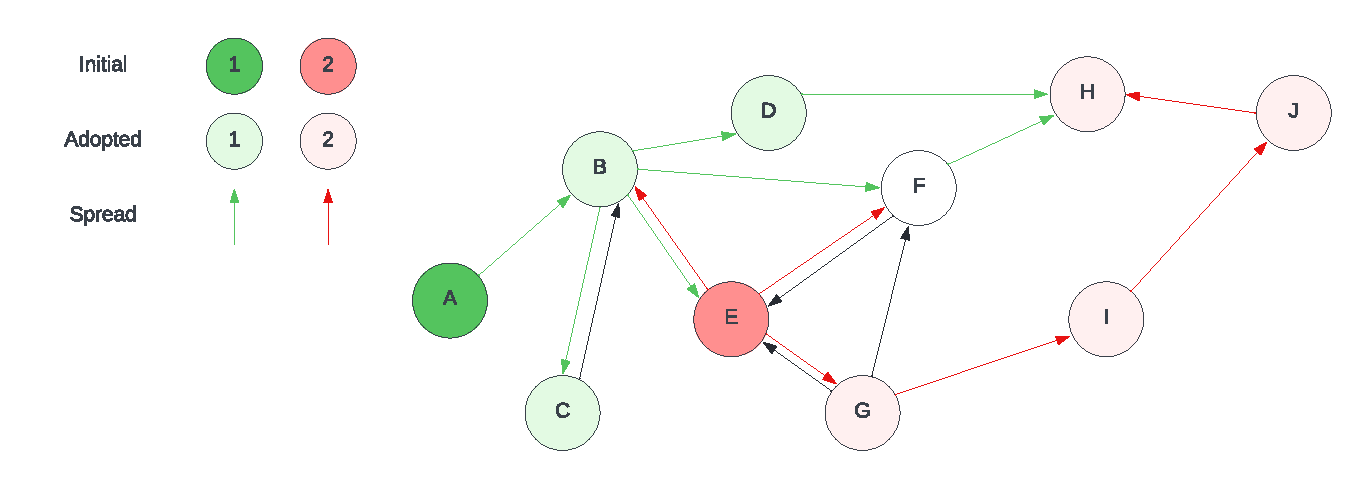
\includegraphics[width=1\linewidth]{graph1.pdf}
    \caption{\textbf{Information Cascade on Directional Social Network}. Individual node has their own belief level $\alpha \in [-1,1]$.}
    \label{fig:1}
\end{figure}
\end{frame}
\section{Spatial-Temporal Influence Maximization in Swarm Robotics}
\begin{frame}{Pheromone-Based Robot Foraging}
\begin{figure}
    \centering
    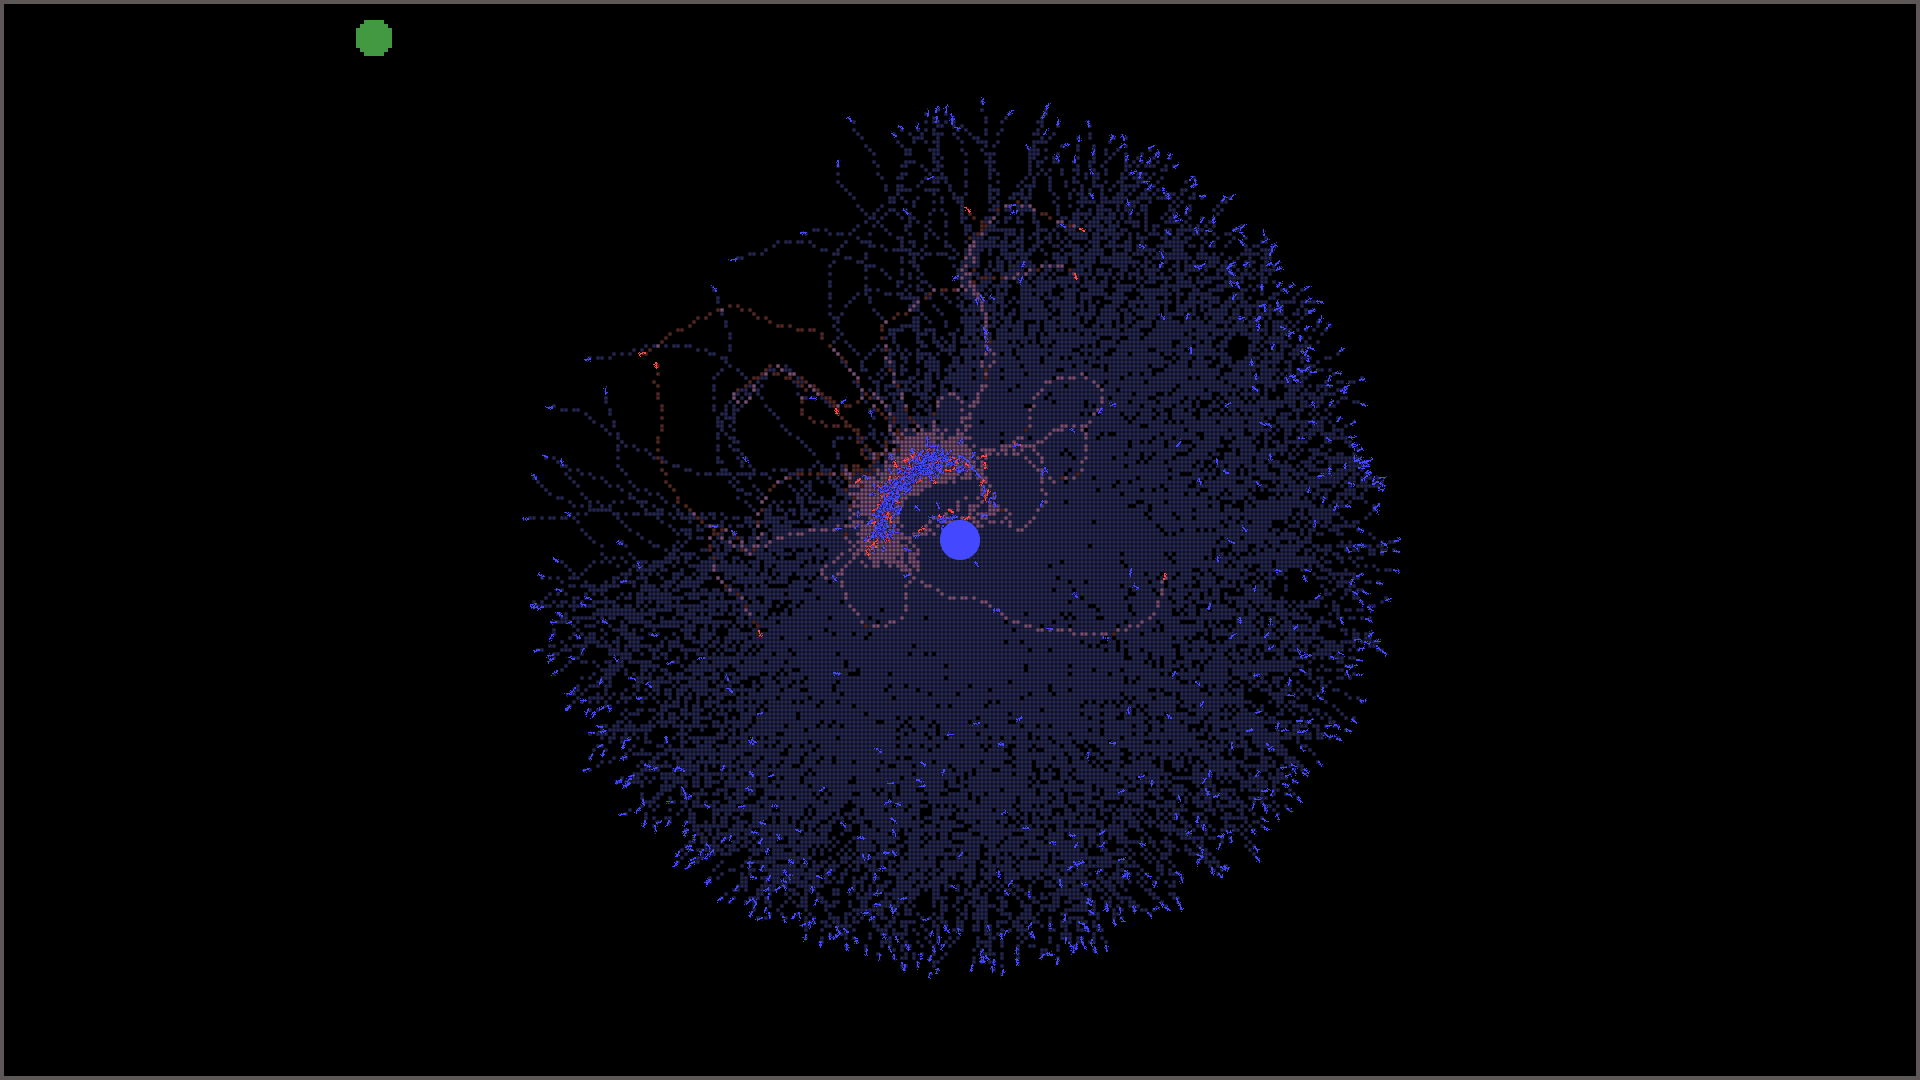
\includegraphics[width=1\linewidth]{DetractorWall.png}
    \caption{\textbf{Effect of Malicious Actor on the Foraging.} Green is food, blue circle is nest. Blue trails is to-food pheromone and red is adversarial to-food pheromone.}
    \label{fig:2}
\end{figure}
\end{frame}
\begin{frame}{Pheromone-Based Robot Foraging: Cautionary Pheromone}
\begin{figure}
    \centering
    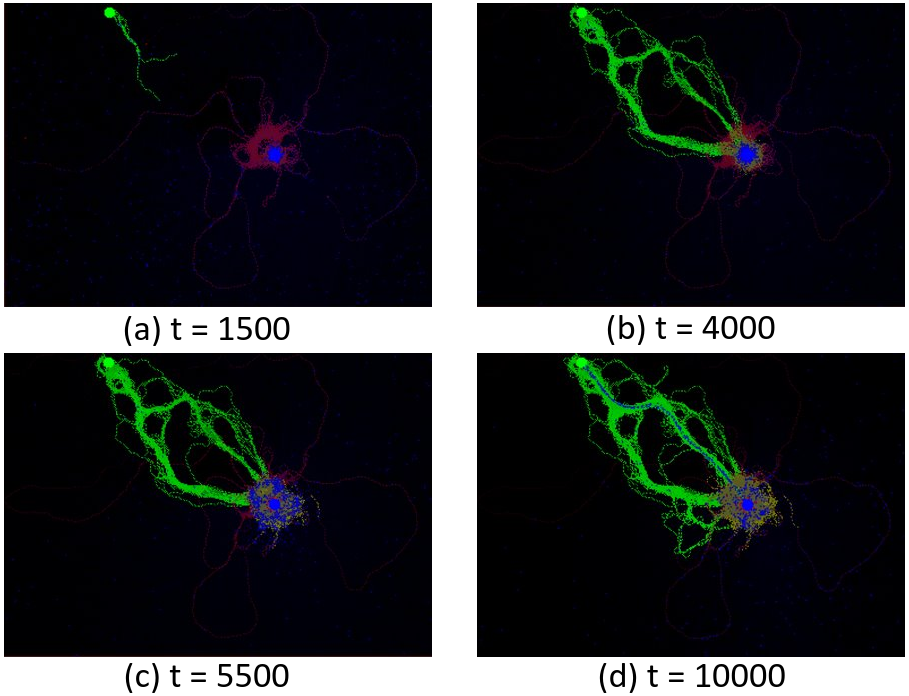
\includegraphics[width=0.8\linewidth]{counter_timeline.png}
    \caption{\textbf{Time Evolution Of Pheromone Concentration Given Cautionary Pheromone} (Aswale et al., AAMAS 2022)}
    \label{fig:2}
\end{figure}
\end{frame}
\begin{frame}{Pheromone and Robot Dynamics}
\begin{itemize}
    \item Suppose $i=1,\dots,N$ are robots that locate at $x_i(t)$. At position $x(t)$, there are 2 pheromones concentration $P_\text{food},P_{\text{home}}$
    \[
    \dd x_i(t) = \overbrace{v_i(t) \dd t}^\text{correlated term} + \underbrace{\sigma \dd W_i(t)}_{\text{random walk}}
    \]
    \[
    \dfrac{\partial}{\partial t} P_\ell(x,t) = \overbrace{D_\ell \nabla^2P_\ell(x,t)}^{\text{diffusion}} - \underbrace{\lambda_\ell P_\ell(x,t)}_{\text{evaporation}} +\overbrace{S_\ell(x,t)}^{\text{deposition}}, \quad \ell\in\{\text{food},\text{home}\}
    \] (Ryan, Journal of Mathematical Biology, 2016)
    \item Note that pheromone dynamics is SPDE as \[S_\ell(x,t) = \sum_{i=1}^N s_i(t)\delta(x-X_i(t))\] for random position $X_i(t)$ described by dynamics $\dd x_i(t)$
    \item Robot has prior belief in trustworthiness of the observation.
\end{itemize}
\end{frame}
\section{Methodology}
\begin{frame}{Method}
    \begin{itemize}
        \item Monte Carlo simulation of different settings as initial dynamics.
        \begin{itemize}
            \item In discrete case, we can look at the Erd\H{o}s-R\'enyi social network with different families of distributions of propagation: uniform, heavy-tailed, Gaussian, etc. Or using the synchronization/quorum sensing as the way to model the dynamics.
            \item Continuous case, we have some prior data and simulator from previous work.
        \end{itemize}
        \item Theoretical exploration
        \begin{itemize}
            \item Both are evolution of distribution which is the solution of SDE (and also PDE). So, Kolmogorov forward equation or Fokker-Planck equation might needed to be considered.
        \end{itemize}
        \item Information Structure
        \begin{itemize}
            \item How would knowing more information (say if robot can communicate, or we know which side that person is on) changes the strategy?
        \end{itemize}
    \end{itemize}
\end{frame}
\section{Theoretical Results}
\begin{frame}{Dynamics as Gradient Flow}
    \begin{itemize}
        \item One can say that the system
        \begin{align}
    \dfrac{\partial}{\partial t} P_\ell(x,t) &= D_\ell \nabla^2P_\ell(x,t) -\lambda_\ell P_\ell(x,t) +S_\ell(x,t)\\
    \dd x_t &= \mu(X_t,t)\dd t + \sigma(X_t,t)\dd W_t\\
    X_t &\sim F(t,\theta) \text{ unknown}
    \end{align}
    can be written as
    \begin{equation}
        \partial_t\eta = \nabla^2\eta + \nabla \cdot \left(\eta (\nabla V+ \nabla W[\mu])\right)
    \end{equation}
    for some measure $\mu$ and potential function $V$ (as gradient flow).
    \end{itemize}
\end{frame}
\begin{frame}{Information Structure}
    \metroset{block=fill}
    \begin{block}{Theorem}
    Pheromone dynamics follows the Blackwell's information structure. 
    \end{block}
    \begin{proof}
        \begin{itemize}
            \item Intuitively, one can see that the dynamic system we discussed is indeed diffusion process with additional term governing the input and output of the system. In a way, we have
            \[
            \dfrac{\partial}{\partial t} P_\ell(x,t) = D_\ell \nabla^2P_\ell(x,t) + f(P_\ell(x,t),x,t)
             \]
            Then, we need to show that there exists the relationship
            \[
            \forall \mu \in \Omega_{\Xi}, \forall\hat{\xi},\tilde{\xi}\in \Xi, \tilde{\xi} = \hat{\xi}D \implies \mu(\hat{\xi}) \leq \mu(\tilde{\xi})
            \]
            for diffusion process $D$.
        \end{itemize}
    \end{proof}
\end{frame}
\begin{frame}{Information Structure (Continue)}
    \metroset{block=fill}
    \begin{proof}
        \begin{itemize}
        \item Note that our pheromone dynamics is (stochastic) parabolic equation satisfying the condition $B^2 + AC = 0$.
        \item It is also in the form of
        \begin{equation}
        \left(\dfrac{\partial}{\partial t}-\mathcal{L}\right) U + qU = F, \quad \left.U\right|_{t=0} = G    
        \end{equation}
        \item Here, we can think of our Laplacian as elliptic operator and our forcing term as random deposition with unknown potential $U$.
        \item There are two dynamics:
        \[
        P_o = P_T + P_A
        \]
        We know $P_o$ and want to recover $P_T$ but we don't know $P_A$
    \end{itemize}
    \end{proof}
    \end{frame}
    \begin{frame}{Another direction}
        \begin{itemize}
            \item NTS that 1 and 2 are equivalent to
            \begin{align*}
            \dd u(t) + [\gamma Au(t)+B(u(t),u(t)) &+F(u(t))]\dd t = G(u(t-))\dd W \\
            &\phantom{=}+ \int_{E_0}K(u(t-),\xi)
            \dd \hat{\pi}(t,\xi)\\
            &\phantom{=}+ \int_{E\setminus E_0}\mathcal{K}(u(t-),\xi)\dd\pi(t,\xi)\\
            &u(0) = u_0
            \end{align*}
            \item $u\in H$ separable (real) Hilbert, $A$ linear operator on $H$ (not necessary bounded), $B$ bilinear form, and $F$ monotone operator over reflexive Banach $X$ densely and continuously embedded in $H$. (Nguyen et al., 2021)
        \end{itemize}
    \end{frame}
    \begin{frame}{Another Direction (continue)}
    \begin{itemize}
    \item Notice that our formulation follows the SPDE with Levy noise. More specifically, it is parabolic SPDE with Levy noise.
    \begin{itemize}
        \item To see this, notice that
        \[
        S_\ell(x,t) = \sum_{k=1}^n s\delta(x-X_i(t)), \dd X_i = \mu \dd t + \sigma \dd W_t 
        \]
        Essentially we are asking if our Ornstein-Uhlenbeck process hit the specific $x$ or not. At the position on some path, if there is ant there, the pheromone level jump (from deposition) rather than decay or diffusion. Hence, acts like Levy noise.
        \item Moreover,
        \[
        \dfrac{\partial}{\partial t}P(x,t) = D\nabla^2P(x,t) - \gamma P(x,t) + S(x,t)
        \]
        is linear, is regularized (in a sense). That is, say if we have $\partial_tP \in L^2$ then, $D\nabla^2P \in W^1$ Sobolev (think of it as linear space of function with $L^p$ norm), more smooth or something. Hence, parabolic (in PDE sense)
    \end{itemize}
    \end{itemize}
    \end{frame}
	\begin{frame}{Adversarials}
		\begin{itemize}
			\item Suppose the dynamics $X_i(t)$ is now defined as
				\[
				\dd X_i = \begin{cases}
				\mu(\nabla P) \dd t + \sigma \dd W_t & \text{ w.p. } p\\
				\sigma \dd W_t & \text{ w.p. } 1-p
				\end{cases}
				\]
			\item Now, we have hidden Bernoulli process.
      \item Goal: Represent $p$ with some dynamics
      \item Moreover, we can argue that there exists $\Lambda = \{\lambda_1,\dots,\lambda_m\}\subseteq \{1,\dots,N\}$ such that for any robot in $\Lambda$, the dynamics for random walk is diffrent compared to the rest of cohort (i.e, adversaries).

		\end{itemize}
	\end{frame}
  \begin{frame}{Model}
    \begin{itemize}
      \item WLOG, there are $N$ robots, $1,\dots, n$ are under normal operation, $n+1, \dots, N$ are faulty (or adversaries).
      \item System follows this dynamics
        \begin{align*}
          \dfrac{\partial}{\partial} P(x,t) &= D\nabla^2 P(x,t) - \gamma P(x,t) + S_n(x,t)+ S_f(x,t)\\
          S_n(x,t) &= \sum_{i=1}^{n}s_n\delta(x-X_i(t))\\
          \dd X_i(t) &= Z_i(t)\left[\mu(\nabla P(X_i,t))\dd t + \sigma \dd W_t\right] + (1-Z_i(t))\sigma\dd W_t\\
          Z_i(t) &\sim \operatorname{Ber}(p(t))\\
          S_f(x,t) &= \sum_{k=n+1}^N s_f \delta(x-Y_k(t))\\
          \dd Y_k(t) &= \varphi(\nabla P(Y_k(t),t),t)\dd t + \eta \dd W_t
        \end{align*}
    \end{itemize}
  \end{frame}
  \begin{frame}{Model (continue)}
  \begin{itemize}
  \item What we don't know
        \begin{itemize}
          \item $n$, how many adversaries.
          \item $Y_k(t)$ dynamics of adversaries.
        \end{itemize}
  \end{itemize}
  \end{frame}
\end{document}
            
